\section{Μοντέλα Κύκλου Ζωής Λογισμικού}

\subsection{Μοντέλο Καταρράκτη}

\begin{figure}[H]
	\centering
	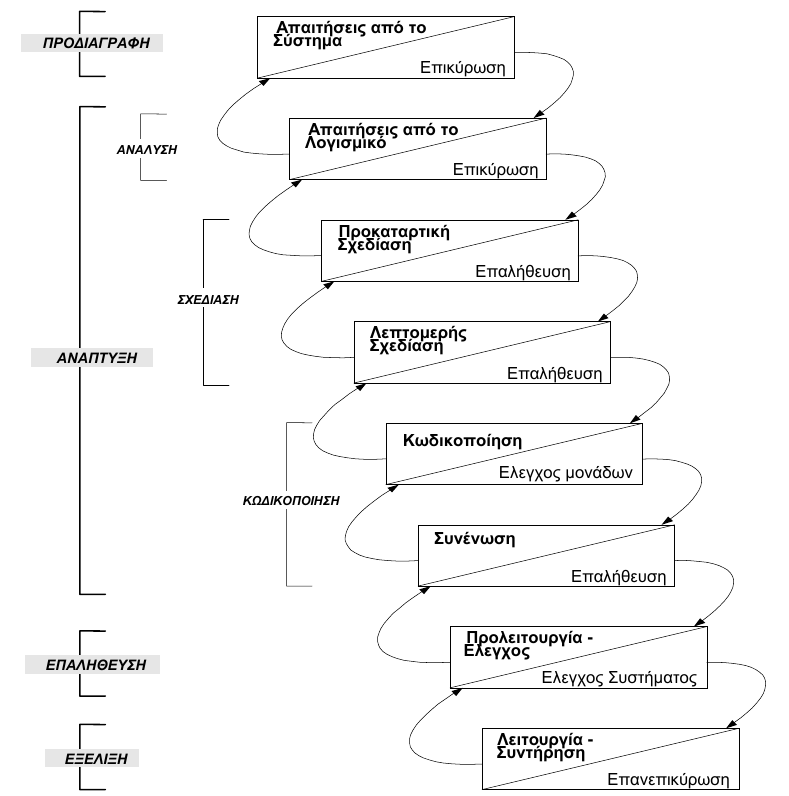
\includegraphics[width=0.6\textwidth]{waterfall.png}
	\caption{Waterfall model}
\end{figure}


\begin{itemize}
	\item	Καλό για μικρού ή μεσαίου μεγέθους εφαρμογές με απαιτήσεις
		εκ των προτέρων γνωστές.
	\item	Πρόβλημα αν αλλάξουν οι απαιτήσεις κατα την κατασκευή.
	\item	Διάδοση μεγάλη με τάσεις μείωσης.
\end{itemize}


\subsection{Μεντέλο Πρωτοτυποποίησης}

\begin{figure}[H]
	\centering
	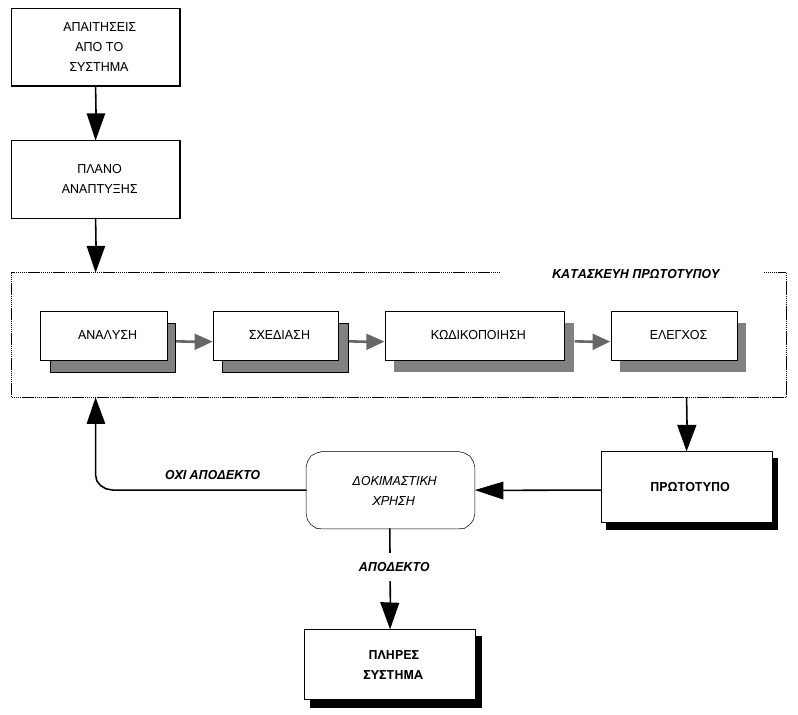
\includegraphics[width=0.6\textwidth]{prototyping.png}
	\caption{Prototyping Model}
\end{figure}

\begin{itemize}
	\item	επαναληπτικό μοντέλο που σε κάθε κύκλο κατασκευάζενται
		διαδοχικά πρότυπα με ολοένα περισσότερα χαρακτηριστικά αυτό να γίνει 
		αποδεκτό από τον πελάτη. Κάθε πρότυπο είναι ένα μικρό έργο λογισμικού 
		και μπορεί να χρησιμοποιεί άλλα μοντέλα.
	\item	ιδανικό για μικρές ή μεσαίες εφαρμογές που οι απαιτήσεις τους δεν είναι από την 
		αρχή γνωστές.
	\item	ιδιαίτερη σημασία αποκτά η διοίκηση του έργου.
	\item	διάδοση μικρή με τάσεις αύξησης
\end{itemize}

\subsection{Μοντέλο Λειτουργικής Επαύξησης}

\begin{figure}[H]
	\centering
	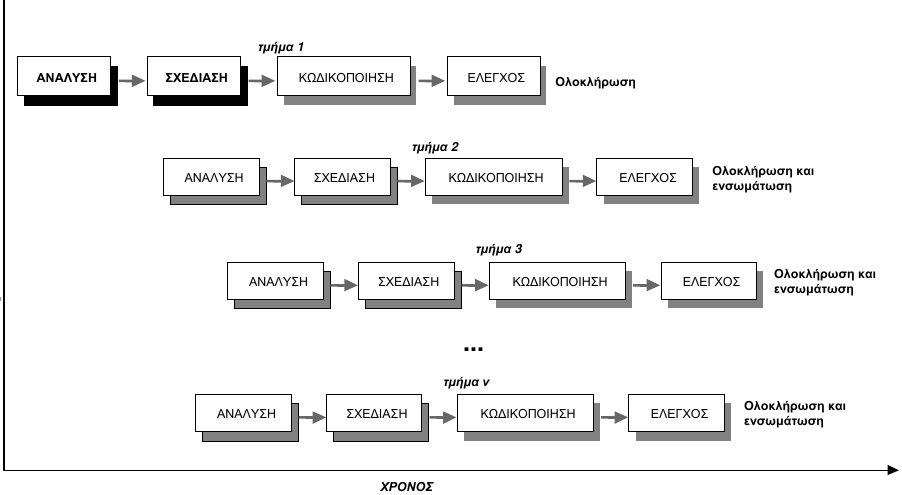
\includegraphics[width=0.6\textwidth]{incremental.png}
	\caption{Incremental Model}
\end{figure}

\begin{itemize}
	\item	Κατάτμηση του λογισμικού, εφαρμογή του μοντέλου του καταράκτη σε κάθε τμήμα και
		συνένωση του στο τέλος.
	\item	πλεονεκτήματα είναι η δυνατότητα παράλληλης ανάπτυξης, η οποία τελικά καταλάμβάνει
		μικρότερο χρόνο, καθώς και ο διαδοχικός εμπλουτισμός των λειτουργικών χαρακτηριστικών του.
	\item	μειονέκτημα: ιδιαίτερη βαρύτητα έχει η αρχική κατάτμηση του λογισμικού.
	\item	μειονέκτημα: Οι μεταβολές στις απαιτήσεις μπορεί να κλονίσουν την ανάπτυξη των υπόλοιπων τμημάτων.
	\item	Μεσαίος ως μεγάλο μέγεθος έργου με σαφείς απαιτήσεις από την αρχή.
	\item	διάδοση μικρή με τάση μείωσης.
\end{itemize}

\subsection{Σπειροειδές Μοντέλο}

\begin{figure}[H]
	\centering
	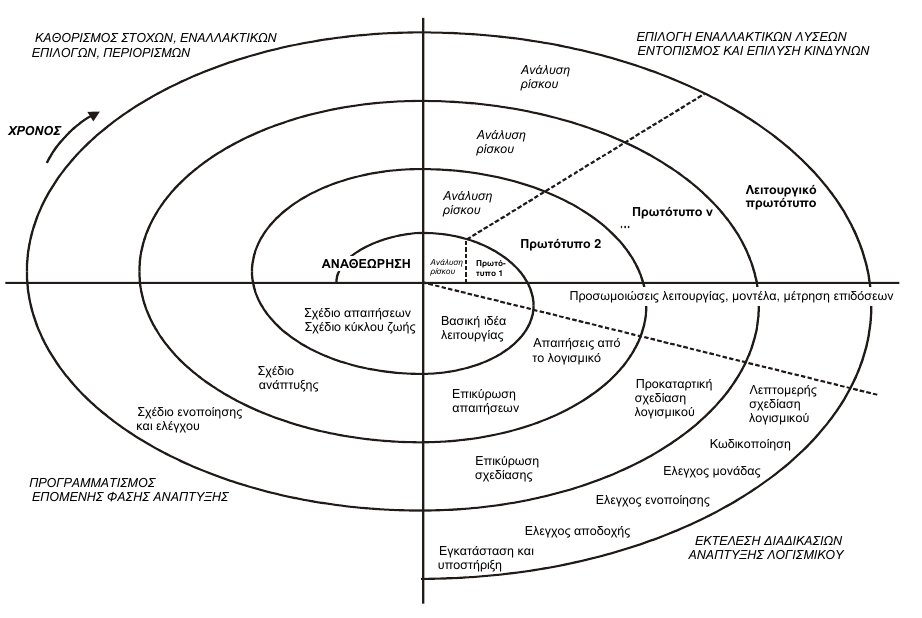
\includegraphics[width=0.6\textwidth]{spiral.png}
	\caption{Spiral Model}
\end{figure}

\begin{itemize}
	\item	Κύκλοι εργασιών με σταδιακή επέκταση των λειτουργικών χαρακτηριστικών της εφαρμογής.
	\item	Εκτίμηση ρίσκου σε κάθε κύκλο.
	\item	Μέγεθος εφαρμογής μεσαίο έως μεγάλο
	\item	Δεκτές οι μεταβολές στις απαιτήσεις
	\item	Αρκετή προσαρμοστικότητα στον κατασκευαστή.
	\item	Διάδοση μικρή με τάσεις μείωσης.
\end{itemize}

\subsection{Μοντέλο Πίδακα}

\begin{figure}[H]
	\centering
	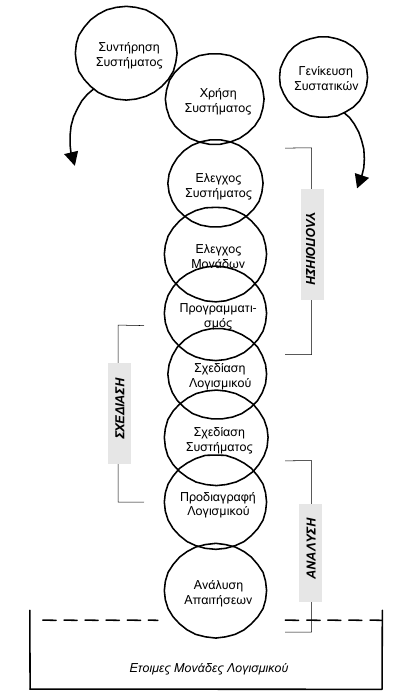
\includegraphics[width=0.6\textwidth]{object_oriented.png}
	\caption{Object Oriented Model}
\end{figure}

\begin{itemize}
	\item	Ανάπτυξη με αντικειμενοστρεφή φιλοσοφία και επαναχρησιμοποίηση έτοιμων συστατικών.
	\item	Κατάλληλο για οποιοδήποτε μέγεθος έργου.
	\item	Δεκτές οι μεταβολές στις απαιτήσεις.
	\item	Αρκετή προσαρμοστικότητα στον κατασκευαστή.
	\item	Διάδοση μικρή.
\end{itemize}

\subsection{Γενικό Μοντελό}

\begin{figure}[H]
	\centering
	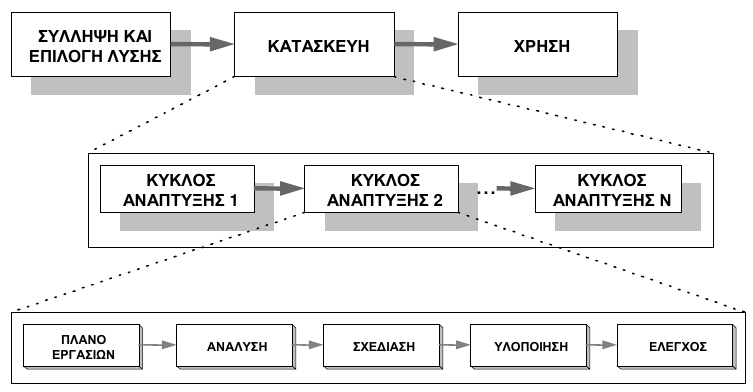
\includegraphics[width=0.6\textwidth]{general.png}
	\caption{General Model}
\end{figure}

\begin{itemize}
	\item	Ανάπτυξη σε κύκλους σύμφωνα με τα χαρακτηριστικά και τις δυνατότητες του κατασκευαστή.
	\item	Γενικευμένη μορφή των προηγούμενων μοντέλων κύκλου ζωής.
	\item	Δεκτές οι μεταβολές στις απαιτήσεις.
	\item	Κατάλληλο για οποιοδήποτε μέγεθος έργου.
	\item	Μεγάλη προσαρμοστικότητα στον κατασκευαστή.
	\item	Διάδοση μικρή με ισχυρές τάσεις αύξησης.
\end{itemize}


\section{Απαιτήσεις από το Λογισμικό}

\begin{itemize}
	\item	Λειτουργικές απαιτήσεις
	\item	Μη λειτουργικές απαιτήσεις
		\begin{itemize}
			\item	Απαιτήσεις χρήσης
			\item	Απαιτήσεις αξιοπιστίας
			\item	Απαιτήσεις επιδόσεων
			\item	Απαιτήσεις υποστήριξης
			\item	Απαιτήσεις σχεδίασης
			\item	Απαιτήσεις υλοποίησης
			\item	Απαιτήσεις επικοινωνίας με άλλα συστήματα
			\item	Απαιτήσεις βάσης δεδομένων
			\item	Φυσικές απαιτήσεις
		\end{itemize}
\end{itemize}

\section{Διάγραμμα Ροής Δεδομένων}

\paragraph{Πηγή ή Αποδέκτης Δεδομένων}
Τα δεδομένα πρέπει πάντοτε να προέρχονται από κάπου και πρέπει να αποστέλλονται σε κάποιον.

\paragraph{Μετασχηματισμός Δεδομένων (αλλάζει την είσοδο σε έξοδο)}
Τα δεδομένα πρέπει πάντοτε να υπόκεινται σε επεξεργασία με
κάποιο τρόπο για να επιτευχθεί η λειτουργία του συστήματος.

\paragraph{Αποθήκη Δεδομένων}
Ο αριθμός των δεδομένων που γράφονται και διαβάζονται πρέπει να είναι ίδιος
στο συνολικό ΔΡΔ.

\begin{itemize}
	\item	Οι ροές εισόδου/εξόδου πρέπει προσεκτικά να καταγράφονται.
	\item	Στο επίπεδο 0 πάντοτε φαίνονται οι εξωτερικές οντότητες (πηγές / αποδέκτες).
	\item	Δώστε ετικέτα σε καθετί.
	\item	Οι εξωτερικές οντότητες μπορεί να επαναλαμβάνονται στο ίδιο διάγραμμα.
	\item	Οι εξωτερικές οντότητες  πρέπει να επαναλαμβάνονται σε όλα τα επίπεδα του ΔΡΔ,
		τουλάχιστον από μία φορά λόγω συνέπειας μεταξύ επιπέδων.
	\item	Κάθε φορά αναλύουμε ένα κύκλο (λειτουργία).
	\item	Η ανάλυση συνεχίζεται μέχρι κάθε κύκλος να αναπαριστά μια απλή και μοναδική λειτουργία 
		που συνδέεται με μια μόνο μονάδα προγράμματος.
	\item	Κάθε ροή δεδομένων (βέλος) μπορεί να αναλύεται στο επόμενο επίπεδο 
		(κάθε ροή δεδομένων καταγράφεται στο λεξικό δεδομένων).
	\item	Δεν περιγράφουμε διαδικαστική λογική (αλγόριθμο).
\end{itemize}

\begin{tabularx}{0.9\textwidth}{|X|X|X|X|}
	\hline
	{} & {Πηγή ή Αποδέκτης} & {Μετασχηματισμός} & {Αποθήκη Δεδομένων} \\
	\hline
	{Πηγή ή Αποδέκτης} & {X} & {\checkmark} & {X} \\
	\hline
	{Μετασχηματισμός} & {\checkmark} & {\checkmark} & {\checkmark} \\
	\hline
	{Αποθήκη Δεδομένων} & {X} & {\checkmark} & {X} \\
	\hline
\end{tabularx}

\begin{figure}[H]
	\centering
	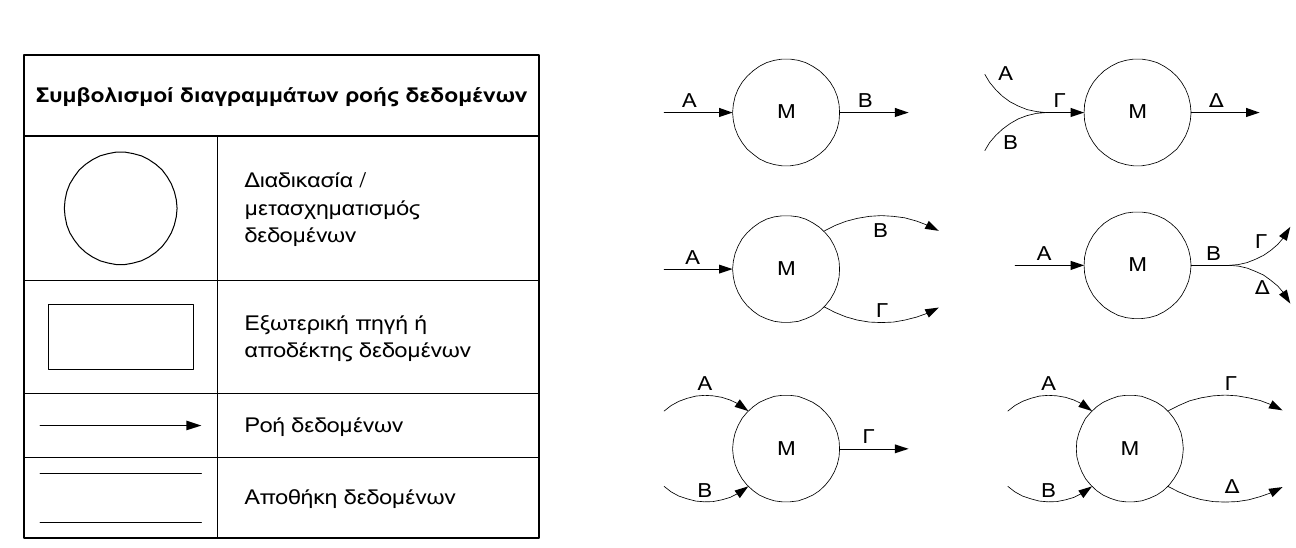
\includegraphics[width=0.9\textwidth]{drd.png}
	\caption{Συμβολισμοί \& Συμβάσεις ΔΡΔ}
\end{figure}


\section{Διάγραμμα Μετάβασης Καταστάσεων}

\begin{figure}[H]
	\centering
	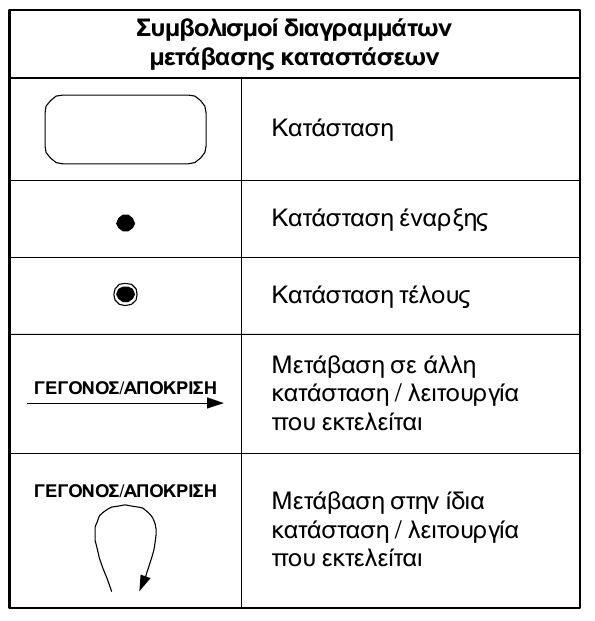
\includegraphics[width=0.5\textwidth]{dmk.png}
	\caption{Συμβολισμοί ΔΜΚ}
\end{figure}

\begin{enumerate}
	\item	Αναγνώριση της οντότητας
	\item	Αναζήτηση γεγονότων/αποκρίσεων
	\item	Αναζήτηση καταστάσεων – Αρίθμησή τους
	\item	Διασύνδεση καταστάσεων - γεγονότων
\end{enumerate}

\section{Λεξικό Δεδομένων}

Ένας πίνακας (ή μια Β.Δ.) που για κάθε στοιχείο δεδομένων περιέχει τουλάχιστον…

\begin{itemize}
	\item	Ονομασία: Το κύριο αναγνωριστικό της οντότητας, πεδίου ή ροής δεδομένων.
	\item	Βοηθητικές ονομασίες: Ονομασίες που χρησιμοποιούνται ισοδύναμα.
	\item	Πού χρησιμοποιείται: Αναφορά στους μετασχηματισμούς, οντότητες κλπ 
		οι οποίοι χρησιμοποιούν το εν λόγω στοιχείο.
	\item	Πώς χρησιμοποιείται: Αναφορά στον τρόπο με τον οποίο χρησιμοποιείται το εν λόγω στοιχείο
		(ως στοιχείο εισόδου, ως αποτέλεσμα, πεδίο, κ.ά.)
	\item	Τι περιέχει: Περιγραφή του είδους και της μορφής της πληροφορίας που αποθηκεύεται σε αυτό.
	\item	Όρια τιμών: Καθορισμός των επιτρεπτών τιμών που μπορεί να πάρει (αν απαιτείται).
	\item	Αρχική τιμή: Καθορισμός της αρχικής τιμής του στοιχείου (αν απαιτείται).
	\item	Λοιπά στοιχεία / συμπληρωματική πληροφορίας: Υπόλοιπες χρήσιμες πληροφορίες.
\end{itemize}

\section{Διάγραμμα Δομής Προγράμματος}

\begin{figure}[Η]
	\centering
	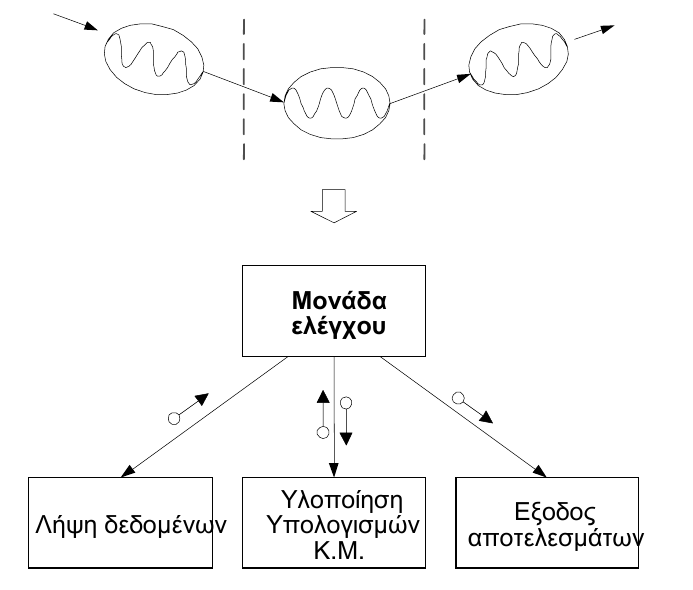
\includegraphics[width=0.4\textwidth]{ddp.png}
	\caption{Παράδειγμα μετατροπής ΚΜ σε ΔΔΠ}
\end{figure}

\begin{enumerate}
	\item	Επιλέγουμε έναν ή περισσότερους μετασχηματισμούς ως κεντρικό μετασχηματισμό.
	\item	Απεικόνιση σε διάγραµµα δοµής προγράµµατος φτιάχνοντας τις κατάλληλες get, put, exec, calc.
		\textbf{Προσοχή} στους σύνθετους κεντρικούς μετασχημάτισμούς μπαίνουν πολλές calc όσοι και
		οι μετασχηματισμοί στο ΔΡΔ.
	\item	Παραγοντοποίηση: επανάληψη για το δεξί και το αριστερό τµήµα του ΚΜ / Κ∆
	\item	Συνένωση τµηµάτων διαγραµµάτων δοµής που προκύπτουν
\end{enumerate}


\section{Διάγραμμα Κλάσεων}

\begin{figure}[H]
	\centering
	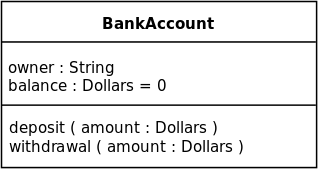
\includegraphics[width=0.4\textwidth]{class.png}
	\caption{Class Example}
\end{figure}

\begin{figure}[H]
	\centering
	
\includegraphics[width=0.4\textwidth]{CD_symbols.png}
	\caption{UML relations notation}
\end{figure}

